
\documentclass[10pt]{report}

% --- Packages ---
\usepackage[utf8]{inputenc}
\usepackage{amsmath, amssymb, amsthm}
\usepackage{geometry}
\usepackage{fancyhdr}
\usepackage{graphicx}
\usepackage{tikz}
\usepackage{enumitem}
\usepackage{hyperref}
\usepackage{xcolor}
\usepackage[framemethod=tikz]{mdframed}
\usepackage{indentfirst}
\usepackage[most]{tcolorbox}
\usepackage{blindtext}
\usepackage{multicol}
\usepackage{paracol}

% --- Page Setup ---
\setlength{\columnsep}{0.6cm}
\geometry{margin=0.6in}
\pagestyle{fancy}
\fancyhf{}
\rhead{Qinghao Hu}
\lhead{SES4U}
\cfoot{\thepage}

% --- Theorem Environments ---
\newtheorem{theorem}{Theorem}[section]
\newtheorem{definition}[theorem]{Definition}
\newtheorem{lemma}[theorem]{Lemma}
\newtheorem{proposition}[theorem]{Proposition}
\newtheorem{corollary}[theorem]{Corollary}
\theoremstyle{remark}
\newtheorem*{remark}{Remark}
\newtheorem*{example}{Example}

% --- Custom Commands ---
\newcommand{\R}{\mathbb{R}}
\newcommand{\N}{\mathbb{N}}
\newcommand{\Z}{\mathbb{Z}}
\newcommand{\Q}{\mathbb{Q}}
\newcommand{\C}{\mathbb{C}}
\newcommand{\ds}{\displaystyle}
\newcommand{\blue}[1]{\textcolor{blue}{#1}}
\newcommand{\red}[1]{\textcolor{red}{#1}}

\newcommand{\mypic}[3]{
    \begin{figure}[h!]
        \centering
        \includegraphics[width=#3\textwidth]{#1}
        \caption{#2}
    \end{figure}
}

\newmdenv[
  backgroundcolor=blue!5,
  linecolor=blue!75!black,
  linewidth=1pt,
  roundcorner=5pt,
  innertopmargin=1mm,
  innerbottommargin=1mm,
  innerrightmargin=2mm,
  innerleftmargin=2mm
]{blueblock}

\newmdenv[
  backgroundcolor=red!5,
  linecolor=red!75!black,
  linewidth=1pt,
  roundcorner=5pt,
  innertopmargin=1mm,
  innerbottommargin=1mm,
  innerrightmargin=2mm,
  innerleftmargin=2mm
]{redblock}

\newmdenv[
  backgroundcolor=green!5,
  linecolor=green!75!black,
  linewidth=1pt,
  roundcorner=5pt,
  innertopmargin=1mm,
  innerbottommargin=1mm,
  innerrightmargin=2mm,
  innerleftmargin=2mm
]{greenblock}

\newmdenv[
  backgroundcolor=cyan!5,
  linecolor=cyan!75!black,
  linewidth=1pt,
  roundcorner=5pt,
  innertopmargin=1mm,
  innerbottommargin=1mm,
  innerrightmargin=2mm,
  innerleftmargin=2mm
]{cyanblock}

\newenvironment{worddef}[1]
  {\par\noindent\textbf{#1:} \itshape}
  {\par\normalfont}
% --- Title ---
\title{\textbf{Grade 12 Earth and Space Science} \\ \large SES4U}
\author{Qinghao Hu}
\date{\today}

\includeonly{chapters/c3}

\begin{document}

\maketitle
\newpage
\tableofcontents
\newpage

\chapter{Unit 1: Astronomy}

\section{Episode 1: Standing up in the Milky Way}
\begin{enumerate}
    \item What is responsible for creating wind and keeping everything in the solar system in its clutches?
    \begin{itemize}
        \item Gravity
    \end{itemize}
    \item What lies between Mars and Jupiter?
    \begin{itemize}
        \item The asteroid belt
    \end{itemize}
    \item What had to be invented before we could discover Saturn and Neptune
    \begin{itemize}
        \item The telescope
    \end{itemize}
    \item What is the name of the spacecraft that has travelled the farthest away from Earth?
    \begin{itemize}
        \item Voyager 1
    \end{itemize}
    \item What is the Oort Cloud?
    \begin{itemize}
        \item A cloud of billions of ice planetesimals surrounding the sun 
    \end{itemize}
    \item What is the "addresss" of Earth in the cosmos?
    \begin{itemize}
        \item Earth, Solar System, Orion Arm, Milky Way, Local Group, Virgo Supercluster, Laniakea Supercluster, Universe
    \end{itemize}
    \item Who was able to prove Giordano Bruno right 10 years after his death?
    \begin{itemize}
        \item Galileo
    \end{itemize}
\end{enumerate}

\section{Episode 4: A Spacetie Odyssey}
\begin{enumerate}
    \item Why do we see the Sun rise before it is over the horizon?
    \begin{itemize}
        \item Because Earth's atmosphere refracts the Sun's image
    \end{itemize}
    \item How far away is Neptune from Earth (in light hours)?
    \begin{itemize}
        \item 4.17 light hours
    \end{itemize}
    \item Using the idea of how fast light travels, how do scientists know our universe is older than 6500 years?
    \begin{itemize}
        \item We know that there are objects farther than 6500 light year away from Earth. 
    \end{itemize}
    \item Why does no one know what happened before the Big Bang?
    \begin{itemize}
        \item No evidence survived
    \end{itemize}
    \item How long after the Big Bang did it take for stars to form?
    \begin{itemize}
        \item Millions of years
    \end{itemize}
    \item What did Einstein call the “rules” that must be obeyed when traveling at high speeds?
    \begin{itemize}
        \item Principle of relativity
    \end{itemize}
\end{enumerate}

\section{Measuing the Universe}

\subsection{Some important constants}
The speed of light $c$:
\[
    c = 3.00 * 10^8\frac{m}{s} (3SD)
\]
The distance of a light year:
\[
    \text{A light year} = 9.4608 * 10^{15} m (3SD)
\]
The distance between \textcolor{red}{Earth} and \textcolor{red}{Sun} refers to the \textit{Astronomicial Unit (AU)}
\[
    AU = 1.4958 * 10^{11}m (3SD)
\]
One Parsec is \textcolor{red}{3.26} light years \[
\text{Parsec} = 3.0824 * 10^{16}m (3SD)
\]

\subsection{Unit Conversion}
\begin{example}
    If 1 inch = 2.54 cm, then 4.5 inches is equivalent to how many cm? \\
    \[
    4.5 \text{ inch } * \frac{2.54cm}{1\text{ }inch} = 11.43 \text{ }cm
    \]
    $\therefore 1 \text{ } inch = 11.43 cm$
\end{example}

\subsection{Radar}
This method is very accurate, it can measure the distance to the moon with an \textcolor{blue}{3 cm} precision!\\

Using radar in Astronomy has some limitations:
\begin{itemize}
    \item Electromagnetic waves tend to \textcolor{blue}{\textit{spread out with distance}} causing weaker signals
    \item The furthest we can measure with this technique is \textcolor{blue}{with a few AUs}
\end{itemize}

\subsection{Parallex}
Parallax refers to how closer objects appear to move compared to farther away objects. This is commonly used in video games
to give the illusion of depth.\\

\mypic{pictures/parallex.png}{Parallax}{0.8}

If we measure the angles that a star shifts using arcseconds, we arrive at how the \textcolor{red}{persec is defined}

\begin{gather}
    d = \frac{1}{p}
\end{gather}

\begin{center}
    $d$ = distance in Parsec\\
    $p$ = parallax angle in arcseconds
\end{center}

\textit{Remainder: The distance that can accurately be measured from the Earth using parallax is \textbf{\textcolor{red}{100}} parsecs.}

\newpage
\section{Cepheid Variable Stars, Redshift and Hubble's Law}
\subsection{Apparent Magnitude and Absolute Magnitude}
In this chapter, I will directly define few terms:

\begin{definition}
   Apparent magnitude = \textit{\textcolor{blue}{How bright an object appears from Earth's surface}}
\end{definition}
\mypic{pictures/ApparentMagnitude.png}{Apparent magnitude (m)}{1}

\begin{definition}
    Absolute Magnitude: How bright an object would appear if it was \textit{\textcolor{blue}{exactly 10 parsecs away}}
\end{definition}

\subsection{Cepheid Variable stars}
\begin{definition}
    Cepheids: Special stars that change how luminous they are at regular time intervals
\end{definition}

Cepheids "pulsate" with \textcolor{blue}{periods} ranging from 1 to 100 days

\subsection{Determining absolute magnitudes using Cepheld Variables}
Absolute magnitudes of stars can be determined using cephelds. It was discovered that period of pulsation is directly related to the star's \textit{lumonosity}

\begin{beamerblock}
    \begin{definition}
         \blue{lumonosity}: The amount of energy emitted by a star each second.
    \end{definition}
\end{beamerblock}

\begin{center}
    \blue{longer} periods have \blue{higher} luminosities
\end{center}

Cepheid Variables are also called "standard candles". Using this method, we can determine distances from 1000 parsecs up to 50 million parsecs

\subsection{Hubble's Law}
Hubble's Law states that:
\begin{center}
    The \blue{further} away and object is, the \blue{faster moving away from us.}
\end{center}

Hubble's law:
\[
    v = Hd
\]
\begin{center}
    $v$ = velocity of object in $km/h$\\
    $d$ = distance in megaparsecs (Mpc)\\
    (1 Mpc = 1 million pc)\\
    $H$ = Hubble's constant
\end{center}

If the velocity of an object is known, we can then calculate their distance.

\subsection{Redshift} 
Luckily, people can determine the the velocity of fast-moving objects with \blue{Redshift}\\
Remember, Doppler Effect causes red shifts
\chapter{Unit 1B}

\section{Proportionality}
\begin{definition}
    Proportionality is concerned witht he relationship between two different variables in an equation. It is the method 
    of showing the \textbf{effective change} in the values of the \textbf{independent variables} will have on the \textbf{dependent variable}
\end{definition}

Proportionality is entirely based on \textbf{multiplication}. If the value of the independent variable is multiplied by a 
\textbf{specific factor}, then the value of the dependent variable will be multiplied by some mathematical operation of that factor. 

\subsubsection*{Direct Proportionality}
In this graph, the proportionality will make a straight line\\

Mathematical expression:
\[
    x \propto y
\]

\subsubsection*{Square Proportionality}
Read "$x$ is proportional to the square of $y$"\\

The graph looks like half of a quadratic function\\

\[
    x \propto y^2
\]

\subsubsection*{Square root proportionality}
Half of a square root function\\

"$x$ is proportional to the square root of $y$"\\

\[
    x \propto \sqrt{y}
\]

\subsubsection*{Inverse square proportionality}
Looks like a rational function\\
\begin{gather*}
    x \propto \frac{1}{y}\\
     x \propto \frac{1}{y^2}\\
      x \propto \frac{1}{y^31}\\
\end{gather*}

\newpage
\section{Fictitious Forces and Apparent Weight}
\subsection{Compare Inertial and non-inertial F.O.R}
\subsubsection{Inertial F.O.R}
One that is not accelerating. It moves at a constant speed\\

\subsubsection{Non-Inertial F.O.R}
This Frame of Reference is accelerating
\subsection{Fictitious Forces}
\red{Fictitious forces} are also called \red{apparent forces} or \red{perceived forces}

\begin{redblock}
    \textbf{Explanation:} When the object is viewed from a \red{non-intertial F.O.R, we created fictitious force to explain the motion and behavior}
\end{redblock}

The \red{fictitious forces} will always act in the direction opposite to the direction of acceleration of 
the frame of reference.\\

\begin{cyanblock}
    The magnitude of each fictitious force can be calculated by:
    \[
        F_{fict} = m|\vec{a_{F.O.R}}|
    \]
\end{cyanblock}

Perceived acceleration could be represented by \red{$\vec{a_{per}}$}

\begin{redblock}
    \textbf{Note: } The object's actual acceleration would be measured relative to an inertial FOR
\end{redblock}

\subsection{Apparent Weight}
Technically, this would be the sum of the \red{normal force} and the force of \red{friction} that a surface exerts 
on an object. In high school, we treat \textit{apparent weight} as just the \textit{normal force a surface exerts}
exerts on the object.

\subsection{Some of the formulas}
\[
    \sum \vec{F} = m\vec{a_{per}}
\]

\newpage
\section{Lecture 2.5}
\subsection{Uniform Circular Motion}
\begin{redblock}
    \textbf{Direction}: The velocity of an object at any point along a circle has a direction that is 
    \red{tangential} to the circle
\end{redblock}

\columnratio{0.6, 0.4}
\begin{paracol}{2}
    \begin{leftcolumn}
        \textbf{Question:} If an object is attached to a string, swung in a circular motion and then the string is released,
        which of the five paths shown here will the object take?\\
        \red{ANS: Path 2}
    \end{leftcolumn}

    \begin{rightcolumn}
        \begin{center}
            \includegraphics[width=0.3\textwidth]{graph/circularMotion.png}
        \end{center}
    \end{rightcolumn}
\end{paracol}

\subsection{Centripetal acceleration}
From the \red{Newton second law}, we understand that \red{An object will accelerate in the same 
direction as the net force}.

If the centripetal force is directed toward the centre of the circle, then what direction is the acceleration in?
\red{ANS: Toward the circle}

In other words, the acceleration will always \red{perpendicular} to the velocity of the object.

\subsection{Formulas}
\begin{cyanblock}
    Formula 1:
    \[
        \vec{a_{c}} = \frac{4 \pi ^2 R}{T^2}
    \]
    \[
        \vec{a_{c}} = 4\pi ^2 R f^2
    \]
    \[
        \vec{a_{c}} = \frac{V^2}{R}
    \]
    \begin{center}
        $\vec{a_{c}}$ is the acceleration of the object in $\frac{m}{s^2}$\\
        $R$ is the radius of the circular path that the object is moving around (in $m$)\\
        $T$ is the period of the object's motion \\
        $v$ is the speed of the object in (m/s)
    \end{center}
\end{cyanblock}

\begin{cyanblock}
    For clockwise:
    \begin{center}
        direction of acceleration = direction of velocity + 90 degree
    \end{center}
    else:
    \begin{center}
         direction of acceleration = direction of velocity - 90 degree
    \end{center}
\end{cyanblock}

\newpage
\section{Motion of a car on Banked Turn}
\begin{center}
    \includegraphics[width=0.7\textwidth]{graph/BankedTurn.png}
\end{center}
\subsection{Forces}
For \red{unbanked Turn}, \red{Static friction} contribute to the centripetal force

For \red{Banked Turn}, both \red{static friction} and \red{normal force} contribute to the centripetal force

\subsection{Critical Speed}
\begin{definition}
    Critical speed the minimum speed needed at which a vehicle can travel around a curve, baked road without relying on static friction
\end{definition}

The formula for critical speed is defined as:
\begin{cyanblock}
    \[
        v = \sqrt{R*tan\theta *g}
    \]
    \begin{center}
        $v$ = Critical Speed\\
        $R$ = The radius of the banked turn\\
        $g$ = The acceleration by Gravity\\
    \end{center}
\end{cyanblock}

Above the \red{critical speed}, the car wants to go \blue{up}. At this case, friction must act \red{down the bank} to prevent sliding outward

Below the \red{critical speed}, the car wants to go \blue{down}. At this case, friction must act \red{up the bank} to prevent sliding inward

\newpage
\section{Universal Gravitation, Gravitational field}
\subsection{Force of Gravity}
The formula for the \textbf{Force of Gravity} acting between two objects is:
\[
    Fg = \frac{G * m_{1} * m_{2}}{R^2}
\]
\begin{center}
    $Fg$ = the magnitude of the force of gravity that $m_{1}$ exerts on $m_{2}$ and $m_{2}$ exerts on $m_{1}$\\
    $G$ = Universal Gravitational Constant\\
    $m_{1}$ = the mass of one of the objects (in kg)\\
    $m_{2}$ = the mass of the other object (in kg)\\
    $R$ is the distance separating the objects' \red{center of mass} in (m)
\end{center}

\red{Remainder:} \textbf{Altitude} refers to the distance between the Earth's surface and the object!\\

In reality, \red{every particle} in A exerts a force of gravity on every particle in B. 
If the objects (A and B) are relatively close together and large (relative to their separation distance)
then these forces are not parallel.
\begin{center}
    \includegraphics[width=0.8\textwidth]{graph/fgparallel.png}
\end{center}

The \textbf{formula works} best for two objects who \red{seperation distance} is \red{very large} relative to their sizes, 
or when both object are perfect \red{sphere}\\

The \textbf{formula works well} for a very, very \red{large} sphere (whose mass is uniformly distributed through out)
and a relatively \red{small} object on its surface\\

You can not use this formula when one object is \red{inside} of another object!

\subsection{Gravational Fields}
\begin{definition}
    \textbf{A force field} is a region surrounding an object in which the object is capable of exerting a force on another object
\end{definition}

A \red{Gravational field} is a region surrounding an object in which the object is capable of exerting a force of gravity 
on another object.

\subsection{Differences between strength of gravity and acceleration}
Acceleration due to gravity:
\begin{center}
    Units: \blue{$\frac{m}{s^2}$}\\
    What does it imply?:  \blue{When an object is in free fall, it will accelerate at that rate}\\
    When is it true: \blue{Only when $Fg$ is the only force on the object}
\end{center}

Gravitational field strength:
\begin{center}
    Units: \blue{$\frac{N}{kg}$}\\
    What does it imply?:  \blue{When an object is in free fall, it will accelerate at that rate}\\
    When is it true: \blue{Gravity is exertings a force of $\mid \vec{g} \mid $ Newtons for each Kg of mass}
\end{center}

Specific types of field strengths are \red{additive}. The \red{net gravitational field strength} at a location is the \red{sum}
of all the individual strengths of gravitational fields at that location OR $\sum \vec{g} = \vec{g_{1}} + \vec{g_{2}}$\\

When you need to calculate \blue{magnitude} of Gravational field from that object $M$ exerts on $m$:
\begin{equation} \label{eq:1}
    Fg_{M/m} = \frac{GMm}{R^2}
\end{equation}
\begin{equation} \label{eq:2}
    Fg_{M/m} = mg
\end{equation}
Add \ref{eq:1} and \ref{eq:2}
\begin{equation}
    g = \frac{GM}{R^2}
\end{equation}
\begin{center}
    $g$ is the \blue{magnitude of the grav field strength} of $M$, at a specific location (in $N/kg$)\\
    $R$ is the distance that the location is from $M$'s centre of mass(in m)\\
    $G$ is the universal gravitational constant ($G$ = $6.67*10^{-11}\frac{Nm^2}{Kg^2}$)
\end{center}

\newpage
\section{Satellites}
A satellite is an object that \red{orbits around another object}\\

There are \textbf{natural} satellites and \textbf{artifical} object
\begin{itemize}
    \item The moon is a \textbf{natural} satellite of the Earth
    \item The international space station (ISS) is an \textbf{artifical} object
\end{itemize}

\subsection{Netwon's Cannon}
His idea was: \textit{if a cannon is placed on the top of a very tall mountain, and if you could ignore air resistance. The cannon 
shoots a cannonball horizontal}\\

At the idea speed: the distance the cannonball has fall \textbf{equals} the distance that the Earth has \textbf{turned away}\\

If $v  < v_{idea}$, the distance between the ball and Earth's surface will \textbf{decrease}\\

If $v  > v_{idea}$, the distance between the ball and Earth's surface will \textbf{increase}\\

The cannon must has a constant speed and travel in the perfect circular path

\subsection{Geosynchronous}
They have the same orbital period as the \textbf{rotational speed} of the object they are on the ground\\

The period is around \textbf{24 hrs}\\

There is a special type of geosynchronous is called \textbf{Geostationary}
\begin{itemize}
    \item "Hang above" a location on Earth's \textbf{Equator}
    \item They orbit in the same \textbf{direction} that the Earth rotates
\end{itemize}

\subsection{Formulas related to satellite}
We will derive each formulas in this handout:\\

To start off, let's draw the FBD for the satellite\\
\begin{center}
    \begin{tikzpicture}[scale=1.2, >=Stealth]

    % Earth
    \shade[ball color=blue!40] (0,0) circle (1);
    \node at (0,0) {\textbf{Earth}};

    % Satellite position
    \coordinate (satellite) at (0,3);
    \filldraw[gray!60] (satellite) circle (0.15);
    \node[above=2pt of satellite] {Satellite};

    % Forces
    \draw[thick, red, ->] (satellite) -- ++(0,-1.2)
        node[midway, right] {$F_g$};
    \draw[thick, blue, ->] (satellite) -- ++(0,1.2)
        node[midway, right] {$F_{\text{fict}}$};

    % Orbit line
    \draw[dashed, gray] (0,0) circle (3);
    \node[right] at (0,1.5) {Orbit altitude};

    % Optional: radius vector
    \draw[->, thick, black!50] (0,0) -- (satellite)
        node[midway, left] {$r$};

    \end{tikzpicture}
\end{center}

\textbf{Down} is negative\\

Let's derive the formula for satellite:
\begin{gather*}
    \sum \vec{F} = m*\vec{a_{per}}\\
    F_g - F_{fict} = 0\\
    mg - m*\left|F_{FOR}\right| = 0\\
    mg = ma_c\\
    a_c = \frac{Gm}{R^2} 
\end{gather*}

Sub in $a_c = \frac{V^2}{R}$:
\begin{gather*}
    \frac{v^2}{R} = \frac{GM}{R^2}\\
    v = \sqrt{\frac{GM}{R}}
\end{gather*}

\begin{center}
    $v$ = orbital speed\\
    $M$ = mass of the object that is obited in (kg)
\end{center}

Sub in $a_c = \frac{4\pi^2 R}{T^2}$
\begin{gather*}
    \frac{4\pi^2 R}{T^2} = \frac{GM}{R}\\
    T^2 = \frac{4\pi^2 R^3}{GM}\\
    T = \sqrt{\frac{4\pi^2 R^3}{GM}}
\end{gather*}

\newpage
\section{Rotating Frame of Reference}
\subsection{Little problem}
When a person is standing (on Earth) there are two forces acting on them:\\

\columnratio{0.4, 0.6}
\begin{paracol}{2}
    \begin{leftcolumn}
        \begin{figure} \label{fig:2.1}
        \centering
            \includegraphics[width=0.2\textwidth]{graph/FBD2.6.1.png}
        \caption{Normal force and Gravity}
        \end{figure}
        
    \end{leftcolumn}

    \begin{rightcolumn}
        The normal force acting on the person is pushing force, thus a force of \textbf{compresion}. An object 
        that has a compression force must be able to \textbf{withstand this force} or it will collapse. (See \ref{fig:2.1})\\

        In the caes of a person, their muscles and their bones must be able to withstand this force, thus you 
        \textbf{muskule-skeletal system develops} to withstand this force
    \end{rightcolumn}
\end{paracol}

When a person is in orbit around a planet, there is only the force of gravity acting on them! They are in 
\textbf{constant state of free fall} \\

FBD for a person orbiting a planet:
\columnratio{0.4, 0.6}
\begin{paracol}{2}
    \begin{leftcolumn}
        \begin{figure}
            \centering
            \includegraphics[width=0.2\textwidth]{graph/FBD2.png}
            \caption{Force of Gravity}
        \end{figure}
    \end{leftcolumn}
    \begin{rightcolumn}
        The person is missing the \textbf{normal force} (the compressive force) that they are used to feeling. 
        Without the compressive force, the person's musculo=skeletal system starts to undergo \textbf{atrophication}
    \end{rightcolumn}
\end{paracol}

To solve this problem, we need to make sure that both two forces are acting on the person. The forces must 
be in \textbf{opposite direction} and one force must be a \textbf{compression force}\\

\subsection*{Solution 1}
The spaceship is \textbf{accelerating} uniformly, in a straight line.\\

But, there are two problems:
\begin{enumerate}
    \item Run out of fuel
    \item As an object speed up, its \textbf{mass increases}. If mass increases, to maintain the acceleration the netforce would also increase
\end{enumerate}

\subsection*{Solution 2}
Get a very very large hallow ring and make it spin\\

For an internal F.O.R, there will be both \textbf{Force of Normal} and \textbf{Force of Gravity} acting on it\\

From an internal F.O.R:
\begin{gather*}
    \sum \vec{F} = m \vec{a_{per}}\\
    F_{N} - F_{fict} = 0\\
    F_{N} = F_{fict}\\
    F_{N} = m*\left| a_{F.O.R}\right| \\
    F_{N} = ma_{c}
\end{gather*}

We can calculate the $v$ of the people:
\begin{gather*} 
    F_{N} = ma_{c}\\
    mg = ma_{c}\\
    g = a_{c}\\
    g = \frac{v^2}{R}\\
    v = \sqrt{gR}
\end{gather*}

So, in the spaceship rotating question, we can always assume:
\begin{equation*}
    F_{N} = F_{g}
\end{equation*}

We can also using
\begin{equation*}
    a_{c} = \frac{4 \pi^2 R}{T^2}
\end{equation*}

To sub in
\begin{gather*}
    g = \frac{4 \pi^2 R}{T^2}\\
    T = \sqrt{\frac{4 \pi^2 R}{g}}
\end{gather*}
or
\begin{equation*}
    f = \sqrt{\frac{g}{4 \pi^2 R}}
\end{equation*}

\subsection{Perceived Acceleration in a Rotating Frame of Reference}
When a person is stand on the equator, there are $a_{c}$ to affect the ball\\

The \textbf{perceived} acceleration should be calculated like this:

\begin{center}
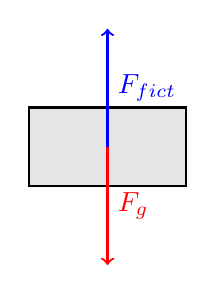
\begin{tikzpicture}[scale=1]
    % Draw the block
    \draw[thick, fill=gray!20] (0,0) rectangle (2,1);
    
    % Draw the surface
    % \draw[thick] (-1,0) -- (3,0);
    
    % Draw the forces
    % Gravity
    \draw[->, thick, red] (1,0.5) -- (1, -1) node[midway, right] {$F_g$};
    % Normal
    \draw[->, thick, blue] (1,0.5) -- (1, 2) node[midway, right] {$F_{fict}$};
    % Friction
    % \draw[->, thick, green] (1,0.5) -- (-1, 0.5) node[midway, above] {$F_f$};
\end{tikzpicture}
\end{center}

Now, let's calculate the $\vec{a_{per}}$
\begin{gather}
    \sum \vec{F} = m\vec{a_{per}}\\
    F_N - F_{fict} = ma_{per}\\
    mg - m\left|a_{F.O.R}\right| = ma_{per}\\
    a_{per} = g - a_c
\end{gather}

\subsection*{Note}
    You can always assume Earth's surface to be an inertial F.O.R unless:
    \begin{itemize}
        \item You need to be \textbf{extremely accurate}
        \item The question states \textbf{at the equator}
    \end{itemize}

\chapter{Earth's Material \& Geological Process}
% \newpage
% \section{Review of Electronstatics}
In this section, we will briefly review basic Electronstatics which we learned from Grade 9 Science

\subsection{Electric Charge}

\subsubsection{Electron}
By the early 1900s, physicists had identified the subatomic particles called the electron and the proton
as the basic units of charge. All protons carry the same amount of positive charge, $e$, and all electrons 
carry an equal but opposite charge, $-e$. Charges interact with each other in very specific ways governed by the 
\textbf{law of electric charges}

\begin{theorem}[Law of Electric Charges]
    Like charges repel each other; unlike charges attract.
\end{theorem}

\noindent\hrulefill

\subsubsection{Charge of atom}
\begin{center}
    Cation: a positive ion. $\#$ of protons $> \#$ of electrons\\
    Anion: a negative ion. $\#$ of protons $< \#$ of electrons\\
\end{center}

The \textbf{Total Charge} is the sum of all the charges in that object and can be positive, negative or zero. The charge is equal to zero when the 
negative charge equals to negative charge. 

\begin{theorem}[Law of Conservation of Charge]
    Charge can be transferred from one object to another, but the total charge of a closed system remains constant. 
\end{theorem}
\noindent\hrulefill

\subsubsection{Coulomb}
The basic unit of charge is called the coulomb (C). The charge of electron, $-e$, is $-1.60*10^{-19}C$, and the charge of a single proton, $+e$, is 
$1.60*10^{-19}C$\\

Symbol $e$ often donotes the magnitude of the charge of an electron or a proton. \\

The symbol $q$ denotes teh amount of charge, such as the total charge onf a small piece of paper. In other words, the total charge of a particle 
is $q$.

% \noindent\hrulefill

\subsection{Conductors and Insulators}
\begin{definition}[Conductor]
    A conductor is a substance in which electrons can move easily among atoms.
\end{definition}

\begin{definition}[Insulator]
    any substance in which electrons are not free to move easily from one atom to another.
\end{definition}

Insulator hold the electron when other electron come in. There are no free electrons in the insulator, and insulator does not allow the extra electrons 
to move about easily. 

% \noindent\hrulefill

\subsection{Different methods of charging}
\subsubsection{Charging an Object by Friction}
In reality, some object has stronger ability to hold on electrons than others. Assume we have two neutral object, when these two objects touch, 
electrons will follow from the object with weaker hold on electrons to the other one with stronger hold on electrons. 

% \noindent\hrulefill

\subsubsection{Carging an object by Induced Charge Separation}
Assume we have two objects, one with zero charge and other one with negative charge. When we put the negative object towards the positive object, 
electrons in the neutral object will repel to the electrons in the negative object. As a result, electrons in the neutral object will redistributed 
throughout the material. The positive side of the netural object is closer than the negative side of the object, in which makes the neutral object 
attrack to the negative object. 

% \noindent\hrulefill
\subsubsection{Charging by Contact}

\begin{figure}[!h]
    \centering
    \includegraphics[width=0.7\textwidth]{pictures/4.1.1.png}
    \caption{Picture from my textbook}
\end{figure}

\subsubsection{Charging by Induction}
\begin{center}
    Using a negative object to create a positive object
\end{center}

\begin{figure}[!h]
    \centering
    \includegraphics[width=0.7\textwidth]{pictures/4.1.2.png}
    \caption{Picture from my textbook}
\end{figure}
% \newpage
% \section{Equations of Motion}
To start off, there are five equations that are used in the calculation of motion
\[
    \vec{v_{f}} = \vec{v_{i}} + \vec{a}*\Delta t
\]
\[
    \Delta\vec{d} = \frac{1}{2}(\vec{v_{i}} + \vec{v_{f}}) * \Delta t
\]
\[
    \Delta\vec{d} = \vec{v_{i}}\Delta t + \frac{1}{2}\vec{a} * \Delta t^2
\]
\[
    \Delta\vec{d} = \vec{v_{f}}\Delta t - \frac{1}{2}\vec{a} * \Delta t^2
\]
\[
    \vec{v_{f}}^2 = \vec{v_{i}}^2 + 2 \vec{a} \Delta \vec{d} 
\]

\subsection{Format requirements for answering Motion questionss}
\begin{enumerate}
    \item You should always include a diagram that contains every known information from the question
    \item $\vec{v}$ should be presented for at least two decimal places
    \item Always list steps in your answer
    \item When using quadratic solving function on calculator, always write \textit{*Using Quadratic Eq} in your answer
    \item When you form an equation system, you should label $1. 2. 3.$ on each equation in the system
    \item Follow the Sig Digit rules
    \begin{itemize}
        \item[!] For \textbf{add} and \textbf{subtract}, keep the least \textbf{decimal places}
        \item[!] For \textbf{multiply} and \textbf{divide}, keep the least amount of \textbf{signficiant digit} 
    \end{itemize}
\end{enumerate}
% \newpage
% \section{Electric Fields}
\begin{definition}[Field]
    The region where an appropriate object would feel a force!
\end{definition}
\begin{itemize}
    \item If there's a gravitational field, a \underline{mass} will feel a force. 
    \item If there's an electric field, a \underline{charge} will feel a force.
    \item If there is an magnetic field, a \underline{magnet} (or a moving charge) will feel a force.
\end{itemize}

Visualizing Electric Fields - Field lines show how a small \underline{\textit{positive}} charge would move.

\begin{figure}[!h]
    \centering
    \includegraphics[width=0.5\textwidth]{pictures/4.3.1.png}
    \caption{Electric field of Positive and negative charge}
\end{figure}

\begin{figure}[!h]
    \centering
    \includegraphics[width=0.5\textwidth]{pictures/4.3.3.png}
    \caption{Electric field between two charges}
\end{figure}

\subsubsection{Parallel Plates}
Two charged metal plates that are parallel to each other $\rightarrow$ "parallel plates"
\begin{itemize}
    \item The field strength outside of the plates is very weak and can be considered negligible
    \item The field lines in between the plates are equdistant stand. 
\end{itemize} 

\subsubsection{Formulas}
\begin{equation}
    \mathcal{E} = \frac{k \left | q \right |}{R^2}
\end{equation}
\begin{center}
    $\mathcal{E}$ is the magnitude of the \underline{electric field strength} around a point charge (in $\tfrac{N}{C}$)\\
    $k = 8.99 \times 10^9 \tfrac{Nm^2}{C^2}$\\
    $R$ is the distance away from the point charge (q) where you want to know the field strength (in $m$)
\end{center}

\noindent\hrulefill
\begin{remark}
    Electric fields are \underline{vector}. The direction of the field will be based on the direction of force that would be 
    exerted on a \underline{positively-charged} object!
\end{remark}
\noindent\hrulefill

\begin{equation}
    \vec{F_E} = q \times \vec{\mathcal{E}}
\end{equation}

\begin{center}
    $\vec{F_E}$ is the magnitude of the electrical force exerted on $q$ (in $N$)\\
    $q$ is the that is \underline{in the electric field}(in $C$)\\
    $\vec{\mathcal{E}}$ is the strength of the electrical field that the charge is in (in $\frac{N}{C}$)
\end{center}
\newpage
\subsection{Continuity and Limits}
\begin{definition}
    [Limits Law]
    Assume we have function $f(x)$ and $g(x)$, which 
    \[
        \lim_{x \to a} f(x) \text{ and } \lim_{x \to a} g(x) \text{ both exist}
    \]
    We also have constant $c$
    We get these properties:
    \begin{enumerate}
        \item \[\lim_{x\to a} c = c\]
        \item \[\lim_{x \to a} x = a\]
        \item \[
            \lim_{x \to a} \left[f(x) + g(x) \right] = \lim_{x \to a} f(x) + \lim_{x \to a} g(x)
        \]
        \item \[
            \lim_{x \to a} \left[f(x) - g(x) \right] = \lim_{x \to a} f(x) - \lim_{x \to a} g(x)
        \]
        \item \[
            \lim_{x \to a} \left[f(x) * g(x) \right] = \lim_{x \to a} f(x) * \lim_{x \to a} g(x)
        \]
        \item \[
            \lim_{x \to a}\frac{f(x)}{g(x)} = \frac{
                \lim_{x \to a} f(x) 
            }{
                \lim_{x \to a} g(x)
            }  
        \]
        \item \[
        \lim_{x \to a} \left[f(x)\right]^n = (\lim_{x \to a}f(x))^n 
        \]
        \item \[
        \lim_{x \to a} \sqrt[n]{f(x)} = \sqrt[n]{(\lim_{x \to a}f(x))} 
        \]
    \end{enumerate}
\end{definition}

Somes cases you should be careful
\begin{example}
    Evaluate and simplify
    \[
        \lim_{x \to a} \sqrt{x}
    \]
    Recall: if a limit exist
    \begin{enumerate}
        \item \[ \lim_{x \to a^{-}} f(x) \text{ exists}\]
        \item \[ \lim_{x \to a^{+}} f(x) \text{ exists}\]
        \item \[ \lim_{x \to a^{-}} f(x) = \lim_{x \to a^{+}} f(x)\]
    \end{enumerate}
    In this case, \[ \lim_{x \to 0^{-}} \sqrt{x} \text{ does not exist}\] because 
    \[
        D: {x \in \mathcal{R} | x \geq 0}
    \]
\end{example}

\begin{example}
    Evaluate and simplify: 
    \[
        \lim_{x \to 1} x^2 - 5x
    \]
    \begin{remark}
        Please be carefull with the bracket, don't mix with 
        \[
            \lim_{x \to 1} (x^2 - 5x)
        \]
    \end{remark}
    The solution should be:
    \begin{gather*}
        = (\lim_{x \to 1}x)^2 - 5x \\
        = (1)^2 - 5x\\
        = 1 - 5x
    \end{gather*}
\end{example}

\end{document}

% Referenc
% \section{Introduction}
% Write your introduction or overview of the day's topic here.
%
% \section{Main Concepts}
% \begin{definition}
% A function \( f: A \to B \) is said to be \textbf{injective} if for every \( a_1, a_2 \in A \), \( f(a_1) = f(a_2) \Rightarrow a_1 = a_2 \).
% \end{definition}
%
% \begin{theorem}
% Let \( f: \R \to \R \) be a continuous and strictly increasing function. Then \( f \) is injective.
% \end{theorem}
%
% \begin{proof}
% Assume \( f(a) = f(b) \). Since \( f \) is strictly increasing, if \( a < b \), then \( f(a) < f(b) \), contradiction. So \( a = b \).
% \end{proof}
%
% \section{Examples}
% \begin{example}
% Let \( f(x) = x^2 \). Then \( f \) is not injective on \( \R \), but it is injective on \( [0, \infty) \).
% \end{example}
%
% \section{Diagrams}
% \begin{center}
% \begin{tikzpicture}[scale=1]
% \draw[->] (-2,0) -- (2,0) node[right] {$x$};
% \draw[->] (0,-1) -- (0,4) node[above] {$y$};
% \draw[domain=-1.5:1.5, smooth, variable=\x, blue, thick] 
%     plot ({\x}, {\x*\x});
% \node at (1.2,3.2) {$y = x^2$};
% \end{tikzpicture}
% \end{center}
%
% \section{Summary}
% Summarize what you learned today.
